\section{Background}
\subsection{Dyck Words}
The language of binary Dyck words is the set of sequences of binary digits that satisfy the following conditions: The sequence has an equal number of ones and zeroes and there is no prefix of the sequence in which the number of zeroes exceeds the number of ones.  The Dyck language can equivalently be thought of as the set of balanced parentheses, with ones representing open parentheses and zeroes representing closing parentheses.  
In addition to balanced parentheses, Dyck words of length $2n$ are also in bijective correspondence with extended binary trees with $n$ internal nodes. 
Given an extended binary tree $B$ with n internal nodes, a Dyck word can be obtained by traversing B in preorder and recording each internal node as a $1$ and each leaf with a $0$, ignoring the final leaf of the tree.

\chapter{Lattice Paths: Lukasiewicz, Motzkin, Schroder}
TODO: this needs to be organized

Motzkin, Schröder, and Łukasiewicz paths provide generalizations of Dyck words.  

Recall the interpretation of Dyck words as paths in the Cartesian plane from Section \ref{sec:Dycks}.

Motzkin paths allow for (1,0) horizontal steps in addition to (1,1) and (1,-1) steps. Schröder paths are identical to Motzkin paths except they allow for $(2,0)$ horizontal steps instead of $(1,0)$.  Łukasiewicz paths allow (1,-1) steps, (1,0) steps and any (1,k) step where k is a positive integer.  All three languages retain the requirement that the path start at the origin, end on the x axis, and never step below the x axis. 

These paths can be encoded in a number of different ways.  In a \emph{-1-based encoding}, each $(1,i)$ step is encoded as i, and every prefix must have a nonnegative sum.  In a \emph{0-based encoding}, each $(1,i)$ step is encoded as $i+1$, and the sum of every prefix must be as large as its length. We primarily use the 0-based encoding. See Fig. \ref{fig:paths}  for examples of these paths using the 0-based encoding.

We refer to Motzkin, Schröder, and Lukasiewicz paths ending at $(n,0)$ as paths of \emph{order n}.  This contrasts slightly with the classification of Dyck words of order n, which terminate at $(2n,0)$

In the context of fixed-content generation, Motzkin and Schröder paths are identical:  Both will have northeast steps encoded as twos, horizontal steps encoded as ones, and southeast steps encoded as zeroes.  However, their Cartesian plane representations will differ in the length of horizontal steps. Notably, Łukasiewicz are a generalization of Motzkin paths, as any Motzkin path is also a Lukasiewicz path.

\begin{figure}[]
	\centering
	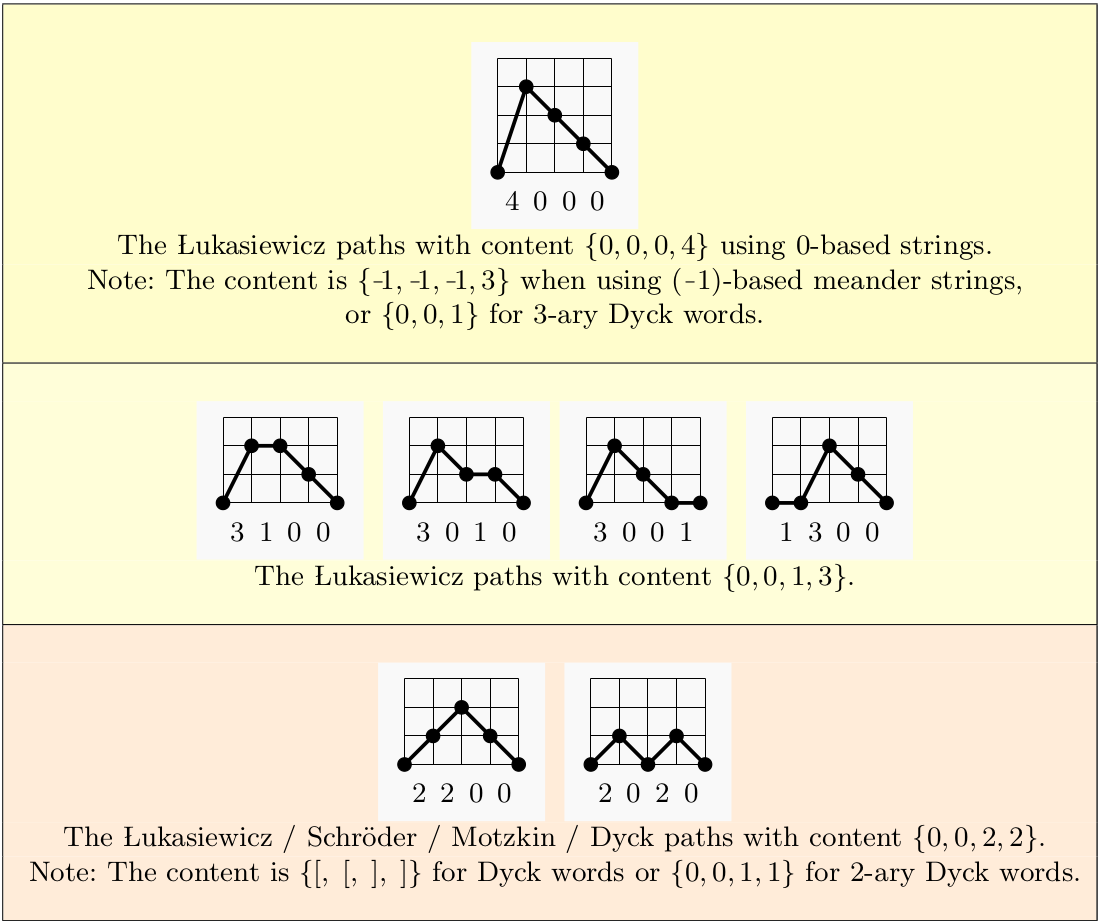
\includegraphics[width = .95 \textwidth]{paths.png}
	\caption{}
	\label{fig:paths}
\end{figure}


The number of Dyck words with n zeroes and n ones are counted by the $n\thh$ Catalan number.  Similarly, the number of Motzkin and Schröder paths of order $n$ are counted by the $n\thh$ Motzkin and big Schröder number respectively. The number of Lukasiewicz paths of order $n$ are counted by the n
Motzkin, Schröder, and Lukasiewicz paths bear a number of interesting bijective correspondences with other combinatorial objects. Richard Stanely's \emph{Catalan Objects} outlines hundreds of interesting examples.  

Lukasiewicz paths  of order $n$ bear a particularly nice correspondence to rooted ordered trees with $n+1$ nodes. See Fig. \ref{trees} for an illustration of this.

\begin{figure}[]
	\centering
	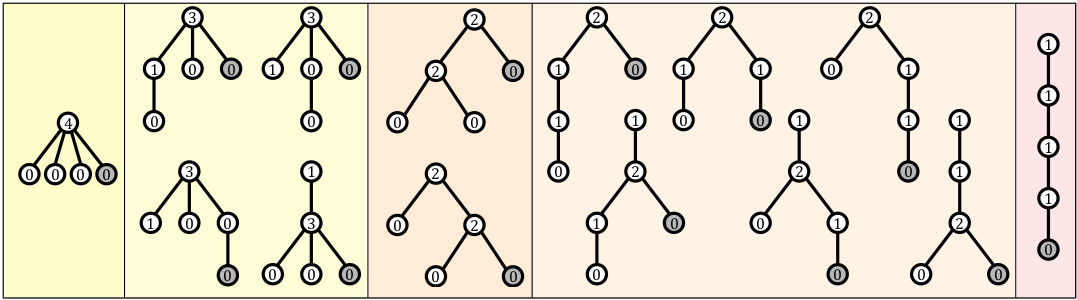
\includegraphics[width = .95 \textwidth]{trees.png}
	\caption{The $\mathcal{C}_4$=14 Lukasiewicz paths of order $n=4$ are in bijective correspondence with the 14 rooted ordered trees with $n+1=5$ nodes.  Given a tree, the corresponding word is obtained by recording the number of children of each node in preorder traversal; the zero from the rightmost leaf is omitted.  For example, the two trees in the middle section correspond to 2200 (top) and 2020 (bottom) respectively.}
	\label{trees}
\end{figure}

% TODO: bijections, mirror chapter 2


This chapter will give background information on cool-lex order and the sets it has been used to enumerate.  
\section{Combinations: Fixed-Weight Binary Strings} \label{sec:coolCombo}
Generating all binary strings with $s$ zeroes and $t$ ones is often referred to as combinations, since each string can be used to represent a choice of $t$ elements from a set of size of $s+t$.  The cool-lex successor rule for generating all fixed-weight binary strings was given by Aaron Williams in his Ph. D thesis and is as follows \cite{williams2009shift}:

\noindent Let $\alpha$ be a binary string of length $n$.

\noindent Let $y$ be the position of the leftmost zero in $\alpha$ and $x$ be the position of the leftmost 1 in $\alpha$ such that $x > y$.  If there is no such 1, let $x=n$.

\noindent Note that $\alpha_1...\alpha_{x-1}$ is the non-increasing prefix of $\alpha$.

\noindent Let $\leftshift[\alpha]{i}$ be a simplified version of the left shift function defined in equation \ref{eq:leftdef}:  $\leftshift[\alpha]{i}$ shifts the $i\thh$ symbol of $\alpha$ into the first position.  Thus, $\leftshift[\alpha]{i}=\lshiftindex[\alpha]{1}{i}$.

% function that shifts the $i\thh$ bit of $\alpha$ into the rotates the first i bits of a string $\alpha$ right circularly by one.

% More formally, 
% \noindent $\leftshift[\alpha]{i}=\alpha_2,\alpha_3,...,\alpha_i,\alpha_1,\alpha_{i-1},\alpha_{i+1},\alpha_{i+2},...,\alpha_{2n}$
\begin{equation*}
    \overleftarrow{\text{cool}}(\alpha) = \begin{cases}
	\leftshift[\alpha]{x} & \text{if $\alpha_{x+1}=1$}\\
	\leftshift[\alpha]{x+1} & otherwise\\
\end{cases}
\end{equation*}

Note that $\alpha_1...\alpha_{x-1}$ must be exactly $1^{y-1}0^{x-y}$, where exponentiation denotes repeated symbols.  Because of this, the two left-shift operations can be replaced with can be replaced with either one or two symbol transpositions.

\noindent Let $\transpose{\alpha}{i}{j}$ with $1 \le i \le j \le n$ be a function that swaps $\alpha_i$ an $\alpha_j$.  More formally, $\transpose{\alpha}{i}{j}=\alpha_1,\alpha_2,\dots,\alpha_{i-1},\alpha_{j}\alpha_{i+1}\dots \alpha_{j-1}\alpha_i \alpha_{j+1}\dots \alpha_n$
The left-shift rule can be re-stated as follows:

\begin{equation*}
    \overleftarrow{\text{cool}}(\alpha) = \begin{cases}
	\transpose{\alpha}{y}{x} & \text{if $\alpha_{x+1}=1$}\\
	\transpose{\transpose{\alpha}{y}{x}}{1}{x+1} & otherwise\\
\end{cases}
\end{equation*}

% To illustrate the first case, consider $\alpha=11001101$; note that x=5. $\leftshift{5}{1}=11100101$ can be accomplished by just setting $\alpha_3=1$ and $\alpha_5=0$, or alternatively $\transpose{\alpha}{3}{5}$

% To illustrate the second case, consider $\alpha=11100101$; note that x=6. $\leftshift{7}{1}=01110011$ with on  can be accomplished by setting $\alpha_4=1$, $\alpha_6=0$, $\alpha_7=1$, and $\alpha_1=0$.  

%Equivalently, the shift can be performed by $\transpose{\transpose{\alpha}{4}{6}}{1}{7}$

% Thus, depending on the value of $\alpha_{x+1}$, the cool-lex successor rule for binary strings requires either one or two transpositions per combination.  

\section{Cool Lex Order on Dyck Paths and Binary Trees}

Ruskey and Williams found the following successor rule for enumerating binary Dyck words, dubbed ``CoolCat" due to its use of a cool-lex order to generate (cat)alan objects \cite{ruskey2008generating}:
We will use $\mathbf{D}_n$ to denote binary Dyck words with $n$ ones and $n$ zeroes.  Note that the length of any string in $\mathbf{D}_n$ is therefore $2n$.

\noindent Let $D \in \mathbf{D}_n$

\noindent Let the $i$th prefix shift of D, denoted by $\preshift{D}{i}$, be a function that rotates the second through $i\thh$ symbols of D one to the right circularly.  More formally, 

\noindent $\preshift{D}{i}=d_1,d_i,d_2,...,d_{i-1},d_{i+1},d_{i+2},...,d_{2n}$

\noindent Note that the prefix shift operation is a special case of the left shift operation defined in $\ref{eq:leftdef}$: $\preshift{D}{i}=\lshiftindex[D]{2}{i}$



\noindent Let $k$ be the index of the 1 in the leftmost $01$ substring in $D$ if it exists and $2n$ if $D$ has no $01$ substring. Note that if $D$ has no $01$ substring, then $D=1^n0^n$.
Furthermore, note that this definition of $k$ is equivalent to the definition of $x$ in \ref{sec:coolCombo}
The successor rule for $D$ is as follows:


\begin{subnumcases}{\coolCat{D} = \label{eq:prefixDyck_simple}}
	% \preshift{D}{2n} & \text{if $D$ has no $01$ substring}\\
	\preshift{D}{k+1} & if $\preshift{D}{k+1} \in \mathbf{D}_n$\\
	\preshift{D}{k} & otherwise
\end{subnumcases}

Ruskey and Williams's algorithm can also enumerate a broader set of strings: The algorithm enumerates any set $\mathbf{D}_{s,t}$ where any $D \in \mathbf{D}_{s,t}$ has s zeroes and t ones and satisfies the constraint that each prefix of D has as many ones as zeroes.  This is slightly broader than the language of Dyck words, as it does not have the requirement that a string have an equal number of ones and zeroes.
We will focus on $\mathbf{D}_n$  languages due to their correspondce with Dyck words and therefore other Catalan objects.

Evaluating whether $\preshift{D}{k+1} \in \mathbf{D}_n$ can be determined by looking at $D_{k+1}$ and the the first $k-1$ symbols of D: 

If $D_{k+1}=1$, then shifting it into the second position is valid.  If $D_{k+1}=0$ and $D$ starts with at least $\frac{k-1}{2}$ ones, then shifting a 0 into the second position will not invalidate the condition that all prefixes of $D$ have at least as many ones as zeroes.   Therefore, the successor rule in \ref{eq:prefixDyck_simple} can be simplified to the following: 

% Let $D'=$ $\preshift{D}{k+1}$

% Note that we know $D \in \mathbf{D}_n$.  

% Since preshift only rotates symbols, $D'$ will automaticallly satisfy the requirement that strings in $\mathbf{D}_n$ must have an equal number of zeroes and ones since D satisfied that requirement. Thus, $D' \in \mathbf{D}_n$ will be determined by whether or not all prefixes of $D'$ have at least as many ones as zeroes.  

% If $D_{k+1}$ is a 1, then  for all i, the $i\thh$ prefix of $D'$ will have at least as many ones as the $i\thh$ prefix of D.  Thus, $D'$ must be $\in \mathbf{D}_n$, as rotating a 1 to earlier in the string will never invalidate the requirement that every prefix of the string has at least as many ones as zeroes.  

% Note that the $k\thh$ prefix of D must be of the form $1^a0^b1$, as otherwise there would be an earlier $01$ prefix.  Fruthermore, $a\ge b$ as otherwise the bth prefix of D would have more zeroes than ones and D would not be a valid Dyck word.

% If $D_{k+1}$ is a 0, then $D' \notin \mathbf{D}_n$ if and only if rotating a 0 to index 2 creates a prefix of D with more zeroes than ones.  This will only happen if the $(k-1)\thh$ prefix of D is exactly $1^{\frac{k-1}{2}}0^{\frac{k-1}{2}}$.  

% Therefore, $\preshift{D}{k+1} \in \mathbf{D}_n \iff D_{k+1}=1$ or $D$ starts with more than $\lfloor \frac{k-1}{2} \rfloor$ ones 

\begin{subnumcases}{\coolCat{D} = \label{eq:prefixDyck}}
    % \preshift{D}{2n} & \text{if $D$ has no $01$ substring} \label{eq:prefixDyck_n}\\
	\preshift{D}{k+1} & $D_{k+1}=1$ or $D$ starts with at least $\lfloor \frac{k-1}{2} \rfloor$ ones \label{eq:prefixDyck_k1}\\
	\preshift{D}{k} & otherwise \label{eq:prefixDyck_k}
\end{subnumcases}


$\preshift{D}{k+1} \in \mathbf{D}_{n} \iff$ $D$ starts with more than $\lfloor \frac{k-1}{2} \rfloor$ ones

Ruskey and Williams provided a loopless pseudocode implementation of CoolCat that utilized this fact to enumerate any $\mathbf{D}_{s,t}$ using at most 2 conditionals per successor \cite{ruskey2008generating}. Using the bijection between Dyck words and binary trees, Ruskey and Williams also showed that their successor rule can be translated to a loopless algorithm for generating all binary trees with $n$ nodes. 

% TODO: binary trees algorithm

Due to its simplicity and efficienty, Don Knuth included the cool-lex algorithm for Dyck words in his 4th volume of \emph{The Art of Computer Programming} and also provided an implementation of it for his theoretical MMIX processor architecture \cite{knuth2015art}.

\section{Multiset Permutations}

Cool-lex order has also been shown to enumerate multiset permutations via prefix shifts.  The rule given by Williams is as follows \cite{williams2009loopless}:

\noindent Let $\alpha$ be a multiset of length $n$.

\noindent Let $i$ be the maximum value such that $\alpha_{j-1} \ge s_j$ for all $2 \le j \le i$.  In other words, $i$ is the length of the non-increasing prefix of $\alpha$.  

Recall the definition of $\leftshift[\alpha]{i}$ from section $\ref{sec:coolCombo}$

% \noindent Let $\sigma_j(\alpha)$ be a function that shifts the $i\thh$ value of $\alpha$ into the first position, or equivalently rotates the first i elements of $\alpha$ right circularly.  More formally, 

% \noindent $\sigma_j(\alpha)=\alpha_j,\alpha_1,\alpha_1,\dots,\alpha_{j-1},\alpha_{j+1},\dots,\alpha_n $

Then

\begin{equation*}
    \text{nextPerm}(\alpha) = \begin{cases}
	\leftshift[\alpha]{i+1} & \text{if $i \le n-2$ and $\alpha_{i+2} > \alpha_i$}\\
	\leftshift[\alpha]{i+2} & \text{if $i \le n-2$ and $\alpha_{i+2} \le \alpha_i$}\\
	\leftshift[\alpha]{n} & otherwise\\
\end{cases}
\end{equation*}


See Fig. \ref{fig:permutations} for an example comparison of cool-lex and lexicographic order for two multisets.

This successor rule has the convenient property of ensuring that length of the successor's non-increasing prefix is easy to find.

In particular, if $\alpha_{i+2}$ is shifted, then the length of the non-increasing prefix is either 1 if $\alpha_{i+2}\le \alpha_1$ or $i+1$ otherwise. 

Similarly, if $\alpha_{i+1}$ is shifted, then the length of the non-increasing prefix is either 1 if $\alpha_{i+1}\le \alpha_1$ or $i+1$ otherwise. 


This property allows for a loopless implementation of the successor rule, as scanning the string to find the length of the non-increasing prefix is not required.  
A similar property regarding the length of successive non-increasing prefixes will allow for a loopless implementation of the shift Gray code for Lukasiewicz words in chapter \ref{chap:luka-implementation}.

Due to the simplicity and efficiency of this rule, it is used in the ``multicool" package in R, which is used for generating multiset permutations, Bell numbers, and other combinatorial objects \cite{multicool_2021}.   Further information on the package is available here: https://www.rdocumentation.org/packages/multicool/versions/0.1-12


\begin{figure}
    \centering

\begin{tabular}{*{4}{c@{\hspace{0.2cm}}c@{\hspace{0.4cm}}}|@{\hspace{0.2cm}}c@{\hspace{0.2cm}}c}


    Cool-Lex & & Lex & & Cool-Lex & & Lex \\
    13221 & \begin{tikzpicture}[scale=30/100]
\fill[fill=p1col1] (0,0) rectangle (0.75,0.4);
\fill[fill=p1col3] (0.9,0) rectangle (1.65,0.9);
\fill[fill=p1col2] (1.7999999999999998,0) rectangle (2.55,0.65);
\fill[fill=p1col2] (2.6999999999999997,0) rectangle (3.4499999999999997,0.65);
\fill[fill=p1col1] (3.5999999999999996,0) rectangle (4.35,0.4);
\end{tikzpicture}
 & 11223 & \begin{tikzpicture}[scale=30/100]
\fill[fill=p1col1] (0,0) rectangle (0.75,0.4);
\fill[fill=p1col1] (0.9,0) rectangle (1.65,0.4);
\fill[fill=p1col2] (1.7999999999999998,0) rectangle (2.55,0.65);
\fill[fill=p1col2] (2.6999999999999997,0) rectangle (3.4499999999999997,0.65);
\fill[fill=p1col3] (3.5999999999999996,0) rectangle (4.35,0.9);
\end{tikzpicture}
 & 1432 & \begin{tikzpicture}[scale=30/100]
\fill[fill=p1col1] (0,0) rectangle (0.75,0.4);
\fill[fill=p1col4] (0.9,0) rectangle (1.65,1.15);
\fill[fill=p1col3] (1.7999999999999998,0) rectangle (2.55,0.9);
\fill[fill=p1col2] (2.6999999999999997,0) rectangle (3.4499999999999997,0.65);
\end{tikzpicture}
 & 1234 & \begin{tikzpicture}[scale=30/100]
\fill[fill=p1col1] (0,0) rectangle (0.75,0.4);
\fill[fill=p1col2] (0.9,0) rectangle (1.65,0.65);
\fill[fill=p1col3] (1.7999999999999998,0) rectangle (2.55,0.9);
\fill[fill=p1col4] (2.6999999999999997,0) rectangle (3.4499999999999997,1.15);
\end{tikzpicture}
 \\ 
    31221 & \begin{tikzpicture}[scale=30/100]
\fill[fill=p1col3] (0,0) rectangle (0.75,0.9);
\fill[fill=p1col1] (0.9,0) rectangle (1.65,0.4);
\fill[fill=p1col2] (1.7999999999999998,0) rectangle (2.55,0.65);
\fill[fill=p1col2] (2.6999999999999997,0) rectangle (3.4499999999999997,0.65);
\fill[fill=p1col1] (3.5999999999999996,0) rectangle (4.35,0.4);
\end{tikzpicture}
 & 11232 & \begin{tikzpicture}[scale=30/100]
\fill[fill=p1col1] (0,0) rectangle (0.75,0.4);
\fill[fill=p1col1] (0.9,0) rectangle (1.65,0.4);
\fill[fill=p1col2] (1.7999999999999998,0) rectangle (2.55,0.65);
\fill[fill=p1col3] (2.6999999999999997,0) rectangle (3.4499999999999997,0.9);
\fill[fill=p1col2] (3.5999999999999996,0) rectangle (4.35,0.65);
\end{tikzpicture}
 & 4132 & \begin{tikzpicture}[scale=30/100]
\fill[fill=p1col4] (0,0) rectangle (0.75,1.15);
\fill[fill=p1col1] (0.9,0) rectangle (1.65,0.4);
\fill[fill=p1col3] (1.7999999999999998,0) rectangle (2.55,0.9);
\fill[fill=p1col2] (2.6999999999999997,0) rectangle (3.4499999999999997,0.65);
\end{tikzpicture}
 & 1243 & \begin{tikzpicture}[scale=30/100]
\fill[fill=p1col1] (0,0) rectangle (0.75,0.4);
\fill[fill=p1col2] (0.9,0) rectangle (1.65,0.65);
\fill[fill=p1col4] (1.7999999999999998,0) rectangle (2.55,1.15);
\fill[fill=p1col3] (2.6999999999999997,0) rectangle (3.4499999999999997,0.9);
\end{tikzpicture}
 \\
    23121 & \begin{tikzpicture}[scale=30/100]
\fill[fill=p1col2] (0,0) rectangle (0.75,0.65);
\fill[fill=p1col3] (0.9,0) rectangle (1.65,0.9);
\fill[fill=p1col1] (1.7999999999999998,0) rectangle (2.55,0.4);
\fill[fill=p1col2] (2.6999999999999997,0) rectangle (3.4499999999999997,0.65);
\fill[fill=p1col1] (3.5999999999999996,0) rectangle (4.35,0.4);
\end{tikzpicture}
 & 11322 & \begin{tikzpicture}[scale=30/100]
\fill[fill=p1col1] (0,0) rectangle (0.75,0.4);
\fill[fill=p1col1] (0.9,0) rectangle (1.65,0.4);
\fill[fill=p1col3] (1.7999999999999998,0) rectangle (2.55,0.9);
\fill[fill=p1col2] (2.6999999999999997,0) rectangle (3.4499999999999997,0.65);
\fill[fill=p1col2] (3.5999999999999996,0) rectangle (4.35,0.65);
\end{tikzpicture}
 & 3412 & \begin{tikzpicture}[scale=30/100]
\fill[fill=p1col3] (0,0) rectangle (0.75,0.9);
\fill[fill=p1col4] (0.9,0) rectangle (1.65,1.15);
\fill[fill=p1col1] (1.7999999999999998,0) rectangle (2.55,0.4);
\fill[fill=p1col2] (2.6999999999999997,0) rectangle (3.4499999999999997,0.65);
\end{tikzpicture}
 & 1324 & \begin{tikzpicture}[scale=30/100]
\fill[fill=p1col1] (0,0) rectangle (0.75,0.4);
\fill[fill=p1col3] (0.9,0) rectangle (1.65,0.9);
\fill[fill=p1col2] (1.7999999999999998,0) rectangle (2.55,0.65);
\fill[fill=p1col4] (2.6999999999999997,0) rectangle (3.4499999999999997,1.15);
\end{tikzpicture}
 \\
    12321 & \begin{tikzpicture}[scale=30/100]
\fill[fill=p1col1] (0,0) rectangle (0.75,0.4);
\fill[fill=p1col2] (0.9,0) rectangle (1.65,0.65);
\fill[fill=p1col3] (1.7999999999999998,0) rectangle (2.55,0.9);
\fill[fill=p1col2] (2.6999999999999997,0) rectangle (3.4499999999999997,0.65);
\fill[fill=p1col1] (3.5999999999999996,0) rectangle (4.35,0.4);
\end{tikzpicture}
 & 12123 & \begin{tikzpicture}[scale=30/100]
\fill[fill=p1col1] (0,0) rectangle (0.75,0.4);
\fill[fill=p1col2] (0.9,0) rectangle (1.65,0.65);
\fill[fill=p1col1] (1.7999999999999998,0) rectangle (2.55,0.4);
\fill[fill=p1col2] (2.6999999999999997,0) rectangle (3.4499999999999997,0.65);
\fill[fill=p1col3] (3.5999999999999996,0) rectangle (4.35,0.9);
\end{tikzpicture}
 & 1342 & \begin{tikzpicture}[scale=30/100]
\fill[fill=p1col1] (0,0) rectangle (0.75,0.4);
\fill[fill=p1col3] (0.9,0) rectangle (1.65,0.9);
\fill[fill=p1col4] (1.7999999999999998,0) rectangle (2.55,1.15);
\fill[fill=p1col2] (2.6999999999999997,0) rectangle (3.4499999999999997,0.65);
\end{tikzpicture}
 & 1342 & \begin{tikzpicture}[scale=30/100]
\fill[fill=p1col1] (0,0) rectangle (0.75,0.4);
\fill[fill=p1col3] (0.9,0) rectangle (1.65,0.9);
\fill[fill=p1col4] (1.7999999999999998,0) rectangle (2.55,1.15);
\fill[fill=p1col2] (2.6999999999999997,0) rectangle (3.4499999999999997,0.65);
\end{tikzpicture}
 \\
    21321 & \begin{tikzpicture}[scale=30/100]
\fill[fill=p1col2] (0,0) rectangle (0.75,0.65);
\fill[fill=p1col1] (0.9,0) rectangle (1.65,0.4);
\fill[fill=p1col3] (1.7999999999999998,0) rectangle (2.55,0.9);
\fill[fill=p1col2] (2.6999999999999997,0) rectangle (3.4499999999999997,0.65);
\fill[fill=p1col1] (3.5999999999999996,0) rectangle (4.35,0.4);
\end{tikzpicture}
 & 12132 & \begin{tikzpicture}[scale=30/100]
\fill[fill=p1col1] (0,0) rectangle (0.75,0.4);
\fill[fill=p1col2] (0.9,0) rectangle (1.65,0.65);
\fill[fill=p1col1] (1.7999999999999998,0) rectangle (2.55,0.4);
\fill[fill=p1col3] (2.6999999999999997,0) rectangle (3.4499999999999997,0.9);
\fill[fill=p1col2] (3.5999999999999996,0) rectangle (4.35,0.65);
\end{tikzpicture}
 & 3142 & \begin{tikzpicture}[scale=30/100]
\fill[fill=p1col3] (0,0) rectangle (0.75,0.9);
\fill[fill=p1col1] (0.9,0) rectangle (1.65,0.4);
\fill[fill=p1col4] (1.7999999999999998,0) rectangle (2.55,1.15);
\fill[fill=p1col2] (2.6999999999999997,0) rectangle (3.4499999999999997,0.65);
\end{tikzpicture}
 & 1423 & \begin{tikzpicture}[scale=30/100]
\fill[fill=p1col1] (0,0) rectangle (0.75,0.4);
\fill[fill=p1col4] (0.9,0) rectangle (1.65,1.15);
\fill[fill=p1col2] (1.7999999999999998,0) rectangle (2.55,0.65);
\fill[fill=p1col3] (2.6999999999999997,0) rectangle (3.4499999999999997,0.9);
\end{tikzpicture}
 \\
    32121 & \begin{tikzpicture}[scale=30/100]
\fill[fill=p1col3] (0,0) rectangle (0.75,0.9);
\fill[fill=p1col2] (0.9,0) rectangle (1.65,0.65);
\fill[fill=p1col1] (1.7999999999999998,0) rectangle (2.55,0.4);
\fill[fill=p1col2] (2.6999999999999997,0) rectangle (3.4499999999999997,0.65);
\fill[fill=p1col1] (3.5999999999999996,0) rectangle (4.35,0.4);
\end{tikzpicture}
 & 12213 & \begin{tikzpicture}[scale=30/100]
\fill[fill=p1col1] (0,0) rectangle (0.75,0.4);
\fill[fill=p1col2] (0.9,0) rectangle (1.65,0.65);
\fill[fill=p1col2] (1.7999999999999998,0) rectangle (2.55,0.65);
\fill[fill=p1col1] (2.6999999999999997,0) rectangle (3.4499999999999997,0.4);
\fill[fill=p1col3] (3.5999999999999996,0) rectangle (4.35,0.9);
\end{tikzpicture}
 & 4312 & \begin{tikzpicture}[scale=30/100]
\fill[fill=p1col4] (0,0) rectangle (0.75,1.15);
\fill[fill=p1col3] (0.9,0) rectangle (1.65,0.9);
\fill[fill=p1col1] (1.7999999999999998,0) rectangle (2.55,0.4);
\fill[fill=p1col2] (2.6999999999999997,0) rectangle (3.4499999999999997,0.65);
\end{tikzpicture}
 & 1432 & \begin{tikzpicture}[scale=30/100]
\fill[fill=p1col1] (0,0) rectangle (0.75,0.4);
\fill[fill=p1col4] (0.9,0) rectangle (1.65,1.15);
\fill[fill=p1col3] (1.7999999999999998,0) rectangle (2.55,0.9);
\fill[fill=p1col2] (2.6999999999999997,0) rectangle (3.4499999999999997,0.65);
\end{tikzpicture}
 \\
    13212 & \begin{tikzpicture}[scale=30/100]
\fill[fill=p1col1] (0,0) rectangle (0.75,0.4);
\fill[fill=p1col3] (0.9,0) rectangle (1.65,0.9);
\fill[fill=p1col2] (1.7999999999999998,0) rectangle (2.55,0.65);
\fill[fill=p1col1] (2.6999999999999997,0) rectangle (3.4499999999999997,0.4);
\fill[fill=p1col2] (3.5999999999999996,0) rectangle (4.35,0.65);
\end{tikzpicture}
 & 12231 & \begin{tikzpicture}[scale=30/100]
\fill[fill=p1col1] (0,0) rectangle (0.75,0.4);
\fill[fill=p1col2] (0.9,0) rectangle (1.65,0.65);
\fill[fill=p1col2] (1.7999999999999998,0) rectangle (2.55,0.65);
\fill[fill=p1col3] (2.6999999999999997,0) rectangle (3.4499999999999997,0.9);
\fill[fill=p1col1] (3.5999999999999996,0) rectangle (4.35,0.4);
\end{tikzpicture}
 & 2431 & \begin{tikzpicture}[scale=30/100]
\fill[fill=p1col2] (0,0) rectangle (0.75,0.65);
\fill[fill=p1col4] (0.9,0) rectangle (1.65,1.15);
\fill[fill=p1col3] (1.7999999999999998,0) rectangle (2.55,0.9);
\fill[fill=p1col1] (2.6999999999999997,0) rectangle (3.4499999999999997,0.4);
\end{tikzpicture}
 & 2134 & \begin{tikzpicture}[scale=30/100]
\fill[fill=p1col2] (0,0) rectangle (0.75,0.65);
\fill[fill=p1col1] (0.9,0) rectangle (1.65,0.4);
\fill[fill=p1col3] (1.7999999999999998,0) rectangle (2.55,0.9);
\fill[fill=p1col4] (2.6999999999999997,0) rectangle (3.4499999999999997,1.15);
\end{tikzpicture}
 \\
    31212 & \begin{tikzpicture}[scale=30/100]
\fill[fill=p1col3] (0,0) rectangle (0.75,0.9);
\fill[fill=p1col1] (0.9,0) rectangle (1.65,0.4);
\fill[fill=p1col2] (1.7999999999999998,0) rectangle (2.55,0.65);
\fill[fill=p1col1] (2.6999999999999997,0) rectangle (3.4499999999999997,0.4);
\fill[fill=p1col2] (3.5999999999999996,0) rectangle (4.35,0.65);
\end{tikzpicture}
 & 12312 & \begin{tikzpicture}[scale=30/100]
\fill[fill=p1col1] (0,0) rectangle (0.75,0.4);
\fill[fill=p1col2] (0.9,0) rectangle (1.65,0.65);
\fill[fill=p1col3] (1.7999999999999998,0) rectangle (2.55,0.9);
\fill[fill=p1col1] (2.6999999999999997,0) rectangle (3.4499999999999997,0.4);
\fill[fill=p1col2] (3.5999999999999996,0) rectangle (4.35,0.65);
\end{tikzpicture}
 & 4231 & \begin{tikzpicture}[scale=30/100]
\fill[fill=p1col4] (0,0) rectangle (0.75,1.15);
\fill[fill=p1col2] (0.9,0) rectangle (1.65,0.65);
\fill[fill=p1col3] (1.7999999999999998,0) rectangle (2.55,0.9);
\fill[fill=p1col1] (2.6999999999999997,0) rectangle (3.4499999999999997,0.4);
\end{tikzpicture}
 & 2143 & \begin{tikzpicture}[scale=30/100]
\fill[fill=p1col2] (0,0) rectangle (0.75,0.65);
\fill[fill=p1col1] (0.9,0) rectangle (1.65,0.4);
\fill[fill=p1col4] (1.7999999999999998,0) rectangle (2.55,1.15);
\fill[fill=p1col3] (2.6999999999999997,0) rectangle (3.4499999999999997,0.9);
\end{tikzpicture}
 \\
    13122 & \begin{tikzpicture}[scale=30/100]
\fill[fill=p1col1] (0,0) rectangle (0.75,0.4);
\fill[fill=p1col3] (0.9,0) rectangle (1.65,0.9);
\fill[fill=p1col1] (1.7999999999999998,0) rectangle (2.55,0.4);
\fill[fill=p1col2] (2.6999999999999997,0) rectangle (3.4499999999999997,0.65);
\fill[fill=p1col2] (3.5999999999999996,0) rectangle (4.35,0.65);
\end{tikzpicture}
 & 12321 & \begin{tikzpicture}[scale=30/100]
\fill[fill=p1col1] (0,0) rectangle (0.75,0.4);
\fill[fill=p1col2] (0.9,0) rectangle (1.65,0.65);
\fill[fill=p1col3] (1.7999999999999998,0) rectangle (2.55,0.9);
\fill[fill=p1col2] (2.6999999999999997,0) rectangle (3.4499999999999997,0.65);
\fill[fill=p1col1] (3.5999999999999996,0) rectangle (4.35,0.4);
\end{tikzpicture}
 & 1423 & \begin{tikzpicture}[scale=30/100]
\fill[fill=p1col1] (0,0) rectangle (0.75,0.4);
\fill[fill=p1col4] (0.9,0) rectangle (1.65,1.15);
\fill[fill=p1col2] (1.7999999999999998,0) rectangle (2.55,0.65);
\fill[fill=p1col3] (2.6999999999999997,0) rectangle (3.4499999999999997,0.9);
\end{tikzpicture}
 & 2314 & \begin{tikzpicture}[scale=30/100]
\fill[fill=p1col2] (0,0) rectangle (0.75,0.65);
\fill[fill=p1col3] (0.9,0) rectangle (1.65,0.9);
\fill[fill=p1col1] (1.7999999999999998,0) rectangle (2.55,0.4);
\fill[fill=p1col4] (2.6999999999999997,0) rectangle (3.4499999999999997,1.15);
\end{tikzpicture}
 \\
    11322 & \begin{tikzpicture}[scale=30/100]
\fill[fill=p1col1] (0,0) rectangle (0.75,0.4);
\fill[fill=p1col1] (0.9,0) rectangle (1.65,0.4);
\fill[fill=p1col3] (1.7999999999999998,0) rectangle (2.55,0.9);
\fill[fill=p1col2] (2.6999999999999997,0) rectangle (3.4499999999999997,0.65);
\fill[fill=p1col2] (3.5999999999999996,0) rectangle (4.35,0.65);
\end{tikzpicture}
 & 13122 & \begin{tikzpicture}[scale=30/100]
\fill[fill=p1col1] (0,0) rectangle (0.75,0.4);
\fill[fill=p1col3] (0.9,0) rectangle (1.65,0.9);
\fill[fill=p1col1] (1.7999999999999998,0) rectangle (2.55,0.4);
\fill[fill=p1col2] (2.6999999999999997,0) rectangle (3.4499999999999997,0.65);
\fill[fill=p1col2] (3.5999999999999996,0) rectangle (4.35,0.65);
\end{tikzpicture}
 & 4123 & \begin{tikzpicture}[scale=30/100]
\fill[fill=p1col4] (0,0) rectangle (0.75,1.15);
\fill[fill=p1col1] (0.9,0) rectangle (1.65,0.4);
\fill[fill=p1col2] (1.7999999999999998,0) rectangle (2.55,0.65);
\fill[fill=p1col3] (2.6999999999999997,0) rectangle (3.4499999999999997,0.9);
\end{tikzpicture}
 & 2341 & \begin{tikzpicture}[scale=30/100]
\fill[fill=p1col2] (0,0) rectangle (0.75,0.65);
\fill[fill=p1col3] (0.9,0) rectangle (1.65,0.9);
\fill[fill=p1col4] (1.7999999999999998,0) rectangle (2.55,1.15);
\fill[fill=p1col1] (2.6999999999999997,0) rectangle (3.4499999999999997,0.4);
\end{tikzpicture}
 \\
    31122 & \begin{tikzpicture}[scale=30/100]
\fill[fill=p1col3] (0,0) rectangle (0.75,0.9);
\fill[fill=p1col1] (0.9,0) rectangle (1.65,0.4);
\fill[fill=p1col1] (1.7999999999999998,0) rectangle (2.55,0.4);
\fill[fill=p1col2] (2.6999999999999997,0) rectangle (3.4499999999999997,0.65);
\fill[fill=p1col2] (3.5999999999999996,0) rectangle (4.35,0.65);
\end{tikzpicture}
 & 13212 & \begin{tikzpicture}[scale=30/100]
\fill[fill=p1col1] (0,0) rectangle (0.75,0.4);
\fill[fill=p1col3] (0.9,0) rectangle (1.65,0.9);
\fill[fill=p1col2] (1.7999999999999998,0) rectangle (2.55,0.65);
\fill[fill=p1col1] (2.6999999999999997,0) rectangle (3.4499999999999997,0.4);
\fill[fill=p1col2] (3.5999999999999996,0) rectangle (4.35,0.65);
\end{tikzpicture}
 & 2413 & \begin{tikzpicture}[scale=30/100]
\fill[fill=p1col2] (0,0) rectangle (0.75,0.65);
\fill[fill=p1col4] (0.9,0) rectangle (1.65,1.15);
\fill[fill=p1col1] (1.7999999999999998,0) rectangle (2.55,0.4);
\fill[fill=p1col3] (2.6999999999999997,0) rectangle (3.4499999999999997,0.9);
\end{tikzpicture}
 & 2413 & \begin{tikzpicture}[scale=30/100]
\fill[fill=p1col2] (0,0) rectangle (0.75,0.65);
\fill[fill=p1col4] (0.9,0) rectangle (1.65,1.15);
\fill[fill=p1col1] (1.7999999999999998,0) rectangle (2.55,0.4);
\fill[fill=p1col3] (2.6999999999999997,0) rectangle (3.4499999999999997,0.9);
\end{tikzpicture}
 \\
    23112 & \begin{tikzpicture}[scale=30/100]
\fill[fill=p1col2] (0,0) rectangle (0.75,0.65);
\fill[fill=p1col3] (0.9,0) rectangle (1.65,0.9);
\fill[fill=p1col1] (1.7999999999999998,0) rectangle (2.55,0.4);
\fill[fill=p1col1] (2.6999999999999997,0) rectangle (3.4499999999999997,0.4);
\fill[fill=p1col2] (3.5999999999999996,0) rectangle (4.35,0.65);
\end{tikzpicture}
 & 13221 & \begin{tikzpicture}[scale=30/100]
\fill[fill=p1col1] (0,0) rectangle (0.75,0.4);
\fill[fill=p1col3] (0.9,0) rectangle (1.65,0.9);
\fill[fill=p1col2] (1.7999999999999998,0) rectangle (2.55,0.65);
\fill[fill=p1col2] (2.6999999999999997,0) rectangle (3.4499999999999997,0.65);
\fill[fill=p1col1] (3.5999999999999996,0) rectangle (4.35,0.4);
\end{tikzpicture}
 & 1243 & \begin{tikzpicture}[scale=30/100]
\fill[fill=p1col1] (0,0) rectangle (0.75,0.4);
\fill[fill=p1col2] (0.9,0) rectangle (1.65,0.65);
\fill[fill=p1col4] (1.7999999999999998,0) rectangle (2.55,1.15);
\fill[fill=p1col3] (2.6999999999999997,0) rectangle (3.4499999999999997,0.9);
\end{tikzpicture}
 & 2431 & \begin{tikzpicture}[scale=30/100]
\fill[fill=p1col2] (0,0) rectangle (0.75,0.65);
\fill[fill=p1col4] (0.9,0) rectangle (1.65,1.15);
\fill[fill=p1col3] (1.7999999999999998,0) rectangle (2.55,0.9);
\fill[fill=p1col1] (2.6999999999999997,0) rectangle (3.4499999999999997,0.4);
\end{tikzpicture}
 \\
    12312 & \begin{tikzpicture}[scale=30/100]
\fill[fill=p1col1] (0,0) rectangle (0.75,0.4);
\fill[fill=p1col2] (0.9,0) rectangle (1.65,0.65);
\fill[fill=p1col3] (1.7999999999999998,0) rectangle (2.55,0.9);
\fill[fill=p1col1] (2.6999999999999997,0) rectangle (3.4499999999999997,0.4);
\fill[fill=p1col2] (3.5999999999999996,0) rectangle (4.35,0.65);
\end{tikzpicture}
 & 21123 & \begin{tikzpicture}[scale=30/100]
\fill[fill=p1col2] (0,0) rectangle (0.75,0.65);
\fill[fill=p1col1] (0.9,0) rectangle (1.65,0.4);
\fill[fill=p1col1] (1.7999999999999998,0) rectangle (2.55,0.4);
\fill[fill=p1col2] (2.6999999999999997,0) rectangle (3.4499999999999997,0.65);
\fill[fill=p1col3] (3.5999999999999996,0) rectangle (4.35,0.9);
\end{tikzpicture}
 & 2143 & \begin{tikzpicture}[scale=30/100]
\fill[fill=p1col2] (0,0) rectangle (0.75,0.65);
\fill[fill=p1col1] (0.9,0) rectangle (1.65,0.4);
\fill[fill=p1col4] (1.7999999999999998,0) rectangle (2.55,1.15);
\fill[fill=p1col3] (2.6999999999999997,0) rectangle (3.4499999999999997,0.9);
\end{tikzpicture}
 & 3124 & \begin{tikzpicture}[scale=30/100]
\fill[fill=p1col3] (0,0) rectangle (0.75,0.9);
\fill[fill=p1col1] (0.9,0) rectangle (1.65,0.4);
\fill[fill=p1col2] (1.7999999999999998,0) rectangle (2.55,0.65);
\fill[fill=p1col4] (2.6999999999999997,0) rectangle (3.4499999999999997,1.15);
\end{tikzpicture}
 \\
    21312 & \begin{tikzpicture}[scale=30/100]
\fill[fill=p1col2] (0,0) rectangle (0.75,0.65);
\fill[fill=p1col1] (0.9,0) rectangle (1.65,0.4);
\fill[fill=p1col3] (1.7999999999999998,0) rectangle (2.55,0.9);
\fill[fill=p1col1] (2.6999999999999997,0) rectangle (3.4499999999999997,0.4);
\fill[fill=p1col2] (3.5999999999999996,0) rectangle (4.35,0.65);
\end{tikzpicture}
 & 21132 & \begin{tikzpicture}[scale=30/100]
\fill[fill=p1col2] (0,0) rectangle (0.75,0.65);
\fill[fill=p1col1] (0.9,0) rectangle (1.65,0.4);
\fill[fill=p1col1] (1.7999999999999998,0) rectangle (2.55,0.4);
\fill[fill=p1col3] (2.6999999999999997,0) rectangle (3.4499999999999997,0.9);
\fill[fill=p1col2] (3.5999999999999996,0) rectangle (4.35,0.65);
\end{tikzpicture}
 & 4213 & \begin{tikzpicture}[scale=30/100]
\fill[fill=p1col4] (0,0) rectangle (0.75,1.15);
\fill[fill=p1col2] (0.9,0) rectangle (1.65,0.65);
\fill[fill=p1col1] (1.7999999999999998,0) rectangle (2.55,0.4);
\fill[fill=p1col3] (2.6999999999999997,0) rectangle (3.4499999999999997,0.9);
\end{tikzpicture}
 & 3142 & \begin{tikzpicture}[scale=30/100]
\fill[fill=p1col3] (0,0) rectangle (0.75,0.9);
\fill[fill=p1col1] (0.9,0) rectangle (1.65,0.4);
\fill[fill=p1col4] (1.7999999999999998,0) rectangle (2.55,1.15);
\fill[fill=p1col2] (2.6999999999999997,0) rectangle (3.4499999999999997,0.65);
\end{tikzpicture}
 \\
    12132 & \begin{tikzpicture}[scale=30/100]
\fill[fill=p1col1] (0,0) rectangle (0.75,0.4);
\fill[fill=p1col2] (0.9,0) rectangle (1.65,0.65);
\fill[fill=p1col1] (1.7999999999999998,0) rectangle (2.55,0.4);
\fill[fill=p1col3] (2.6999999999999997,0) rectangle (3.4499999999999997,0.9);
\fill[fill=p1col2] (3.5999999999999996,0) rectangle (4.35,0.65);
\end{tikzpicture}
 & 21213 & \begin{tikzpicture}[scale=30/100]
\fill[fill=p1col2] (0,0) rectangle (0.75,0.65);
\fill[fill=p1col1] (0.9,0) rectangle (1.65,0.4);
\fill[fill=p1col2] (1.7999999999999998,0) rectangle (2.55,0.65);
\fill[fill=p1col1] (2.6999999999999997,0) rectangle (3.4499999999999997,0.4);
\fill[fill=p1col3] (3.5999999999999996,0) rectangle (4.35,0.9);
\end{tikzpicture}
 & 3421 & \begin{tikzpicture}[scale=30/100]
\fill[fill=p1col3] (0,0) rectangle (0.75,0.9);
\fill[fill=p1col4] (0.9,0) rectangle (1.65,1.15);
\fill[fill=p1col2] (1.7999999999999998,0) rectangle (2.55,0.65);
\fill[fill=p1col1] (2.6999999999999997,0) rectangle (3.4499999999999997,0.4);
\end{tikzpicture}
 & 3214 & \begin{tikzpicture}[scale=30/100]
\fill[fill=p1col3] (0,0) rectangle (0.75,0.9);
\fill[fill=p1col2] (0.9,0) rectangle (1.65,0.65);
\fill[fill=p1col1] (1.7999999999999998,0) rectangle (2.55,0.4);
\fill[fill=p1col4] (2.6999999999999997,0) rectangle (3.4499999999999997,1.15);
\end{tikzpicture}
 \\
    11232 & \begin{tikzpicture}[scale=30/100]
\fill[fill=p1col1] (0,0) rectangle (0.75,0.4);
\fill[fill=p1col1] (0.9,0) rectangle (1.65,0.4);
\fill[fill=p1col2] (1.7999999999999998,0) rectangle (2.55,0.65);
\fill[fill=p1col3] (2.6999999999999997,0) rectangle (3.4499999999999997,0.9);
\fill[fill=p1col2] (3.5999999999999996,0) rectangle (4.35,0.65);
\end{tikzpicture}
 & 21231 & \begin{tikzpicture}[scale=30/100]
\fill[fill=p1col2] (0,0) rectangle (0.75,0.65);
\fill[fill=p1col1] (0.9,0) rectangle (1.65,0.4);
\fill[fill=p1col2] (1.7999999999999998,0) rectangle (2.55,0.65);
\fill[fill=p1col3] (2.6999999999999997,0) rectangle (3.4499999999999997,0.9);
\fill[fill=p1col1] (3.5999999999999996,0) rectangle (4.35,0.4);
\end{tikzpicture}
 & 2341 & \begin{tikzpicture}[scale=30/100]
\fill[fill=p1col2] (0,0) rectangle (0.75,0.65);
\fill[fill=p1col3] (0.9,0) rectangle (1.65,0.9);
\fill[fill=p1col4] (1.7999999999999998,0) rectangle (2.55,1.15);
\fill[fill=p1col1] (2.6999999999999997,0) rectangle (3.4499999999999997,0.4);
\end{tikzpicture}
 & 3241 & \begin{tikzpicture}[scale=30/100]
\fill[fill=p1col3] (0,0) rectangle (0.75,0.9);
\fill[fill=p1col2] (0.9,0) rectangle (1.65,0.65);
\fill[fill=p1col4] (1.7999999999999998,0) rectangle (2.55,1.15);
\fill[fill=p1col1] (2.6999999999999997,0) rectangle (3.4499999999999997,0.4);
\end{tikzpicture}
 \\
    21132 & \begin{tikzpicture}[scale=30/100]
\fill[fill=p1col2] (0,0) rectangle (0.75,0.65);
\fill[fill=p1col1] (0.9,0) rectangle (1.65,0.4);
\fill[fill=p1col1] (1.7999999999999998,0) rectangle (2.55,0.4);
\fill[fill=p1col3] (2.6999999999999997,0) rectangle (3.4499999999999997,0.9);
\fill[fill=p1col2] (3.5999999999999996,0) rectangle (4.35,0.65);
\end{tikzpicture}
 & 21312 & \begin{tikzpicture}[scale=30/100]
\fill[fill=p1col2] (0,0) rectangle (0.75,0.65);
\fill[fill=p1col1] (0.9,0) rectangle (1.65,0.4);
\fill[fill=p1col3] (1.7999999999999998,0) rectangle (2.55,0.9);
\fill[fill=p1col1] (2.6999999999999997,0) rectangle (3.4499999999999997,0.4);
\fill[fill=p1col2] (3.5999999999999996,0) rectangle (4.35,0.65);
\end{tikzpicture}
 & 3241 & \begin{tikzpicture}[scale=30/100]
\fill[fill=p1col3] (0,0) rectangle (0.75,0.9);
\fill[fill=p1col2] (0.9,0) rectangle (1.65,0.65);
\fill[fill=p1col4] (1.7999999999999998,0) rectangle (2.55,1.15);
\fill[fill=p1col1] (2.6999999999999997,0) rectangle (3.4499999999999997,0.4);
\end{tikzpicture}
 & 3412 & \begin{tikzpicture}[scale=30/100]
\fill[fill=p1col3] (0,0) rectangle (0.75,0.9);
\fill[fill=p1col4] (0.9,0) rectangle (1.65,1.15);
\fill[fill=p1col1] (1.7999999999999998,0) rectangle (2.55,0.4);
\fill[fill=p1col2] (2.6999999999999997,0) rectangle (3.4499999999999997,0.65);
\end{tikzpicture}
 \\
    32112 & \begin{tikzpicture}[scale=30/100]
\fill[fill=p1col3] (0,0) rectangle (0.75,0.9);
\fill[fill=p1col2] (0.9,0) rectangle (1.65,0.65);
\fill[fill=p1col1] (1.7999999999999998,0) rectangle (2.55,0.4);
\fill[fill=p1col1] (2.6999999999999997,0) rectangle (3.4499999999999997,0.4);
\fill[fill=p1col2] (3.5999999999999996,0) rectangle (4.35,0.65);
\end{tikzpicture}
 & 21321 & \begin{tikzpicture}[scale=30/100]
\fill[fill=p1col2] (0,0) rectangle (0.75,0.65);
\fill[fill=p1col1] (0.9,0) rectangle (1.65,0.4);
\fill[fill=p1col3] (1.7999999999999998,0) rectangle (2.55,0.9);
\fill[fill=p1col2] (2.6999999999999997,0) rectangle (3.4499999999999997,0.65);
\fill[fill=p1col1] (3.5999999999999996,0) rectangle (4.35,0.4);
\end{tikzpicture}
 & 1324 & \begin{tikzpicture}[scale=30/100]
\fill[fill=p1col1] (0,0) rectangle (0.75,0.4);
\fill[fill=p1col3] (0.9,0) rectangle (1.65,0.9);
\fill[fill=p1col2] (1.7999999999999998,0) rectangle (2.55,0.65);
\fill[fill=p1col4] (2.6999999999999997,0) rectangle (3.4499999999999997,1.15);
\end{tikzpicture}
 & 3421 & \begin{tikzpicture}[scale=30/100]
\fill[fill=p1col3] (0,0) rectangle (0.75,0.9);
\fill[fill=p1col4] (0.9,0) rectangle (1.65,1.15);
\fill[fill=p1col2] (1.7999999999999998,0) rectangle (2.55,0.65);
\fill[fill=p1col1] (2.6999999999999997,0) rectangle (3.4499999999999997,0.4);
\end{tikzpicture}
 \\
    23211 & \begin{tikzpicture}[scale=30/100]
\fill[fill=p1col2] (0,0) rectangle (0.75,0.65);
\fill[fill=p1col3] (0.9,0) rectangle (1.65,0.9);
\fill[fill=p1col2] (1.7999999999999998,0) rectangle (2.55,0.65);
\fill[fill=p1col1] (2.6999999999999997,0) rectangle (3.4499999999999997,0.4);
\fill[fill=p1col1] (3.5999999999999996,0) rectangle (4.35,0.4);
\end{tikzpicture}
 & 22113 & \begin{tikzpicture}[scale=30/100]
\fill[fill=p1col2] (0,0) rectangle (0.75,0.65);
\fill[fill=p1col2] (0.9,0) rectangle (1.65,0.65);
\fill[fill=p1col1] (1.7999999999999998,0) rectangle (2.55,0.4);
\fill[fill=p1col1] (2.6999999999999997,0) rectangle (3.4499999999999997,0.4);
\fill[fill=p1col3] (3.5999999999999996,0) rectangle (4.35,0.9);
\end{tikzpicture}
 & 3124 & \begin{tikzpicture}[scale=30/100]
\fill[fill=p1col3] (0,0) rectangle (0.75,0.9);
\fill[fill=p1col1] (0.9,0) rectangle (1.65,0.4);
\fill[fill=p1col2] (1.7999999999999998,0) rectangle (2.55,0.65);
\fill[fill=p1col4] (2.6999999999999997,0) rectangle (3.4499999999999997,1.15);
\end{tikzpicture}
 & 4123 & \begin{tikzpicture}[scale=30/100]
\fill[fill=p1col4] (0,0) rectangle (0.75,1.15);
\fill[fill=p1col1] (0.9,0) rectangle (1.65,0.4);
\fill[fill=p1col2] (1.7999999999999998,0) rectangle (2.55,0.65);
\fill[fill=p1col3] (2.6999999999999997,0) rectangle (3.4499999999999997,0.9);
\end{tikzpicture}
 \\
    22311 & \begin{tikzpicture}[scale=30/100]
\fill[fill=p1col2] (0,0) rectangle (0.75,0.65);
\fill[fill=p1col2] (0.9,0) rectangle (1.65,0.65);
\fill[fill=p1col3] (1.7999999999999998,0) rectangle (2.55,0.9);
\fill[fill=p1col1] (2.6999999999999997,0) rectangle (3.4499999999999997,0.4);
\fill[fill=p1col1] (3.5999999999999996,0) rectangle (4.35,0.4);
\end{tikzpicture}
 & 22131 & \begin{tikzpicture}[scale=30/100]
\fill[fill=p1col2] (0,0) rectangle (0.75,0.65);
\fill[fill=p1col2] (0.9,0) rectangle (1.65,0.65);
\fill[fill=p1col1] (1.7999999999999998,0) rectangle (2.55,0.4);
\fill[fill=p1col3] (2.6999999999999997,0) rectangle (3.4499999999999997,0.9);
\fill[fill=p1col1] (3.5999999999999996,0) rectangle (4.35,0.4);
\end{tikzpicture}
 & 2314 & \begin{tikzpicture}[scale=30/100]
\fill[fill=p1col2] (0,0) rectangle (0.75,0.65);
\fill[fill=p1col3] (0.9,0) rectangle (1.65,0.9);
\fill[fill=p1col1] (1.7999999999999998,0) rectangle (2.55,0.4);
\fill[fill=p1col4] (2.6999999999999997,0) rectangle (3.4499999999999997,1.15);
\end{tikzpicture}
 & 4132 & \begin{tikzpicture}[scale=30/100]
\fill[fill=p1col4] (0,0) rectangle (0.75,1.15);
\fill[fill=p1col1] (0.9,0) rectangle (1.65,0.4);
\fill[fill=p1col3] (1.7999999999999998,0) rectangle (2.55,0.9);
\fill[fill=p1col2] (2.6999999999999997,0) rectangle (3.4499999999999997,0.65);
\end{tikzpicture}
 \\
    12231 & \begin{tikzpicture}[scale=30/100]
\fill[fill=p1col1] (0,0) rectangle (0.75,0.4);
\fill[fill=p1col2] (0.9,0) rectangle (1.65,0.65);
\fill[fill=p1col2] (1.7999999999999998,0) rectangle (2.55,0.65);
\fill[fill=p1col3] (2.6999999999999997,0) rectangle (3.4499999999999997,0.9);
\fill[fill=p1col1] (3.5999999999999996,0) rectangle (4.35,0.4);
\end{tikzpicture}
 & 22311 & \begin{tikzpicture}[scale=30/100]
\fill[fill=p1col2] (0,0) rectangle (0.75,0.65);
\fill[fill=p1col2] (0.9,0) rectangle (1.65,0.65);
\fill[fill=p1col3] (1.7999999999999998,0) rectangle (2.55,0.9);
\fill[fill=p1col1] (2.6999999999999997,0) rectangle (3.4499999999999997,0.4);
\fill[fill=p1col1] (3.5999999999999996,0) rectangle (4.35,0.4);
\end{tikzpicture}
 & 1234 & \begin{tikzpicture}[scale=30/100]
\fill[fill=p1col1] (0,0) rectangle (0.75,0.4);
\fill[fill=p1col2] (0.9,0) rectangle (1.65,0.65);
\fill[fill=p1col3] (1.7999999999999998,0) rectangle (2.55,0.9);
\fill[fill=p1col4] (2.6999999999999997,0) rectangle (3.4499999999999997,1.15);
\end{tikzpicture}
 & 4213 & \begin{tikzpicture}[scale=30/100]
\fill[fill=p1col4] (0,0) rectangle (0.75,1.15);
\fill[fill=p1col2] (0.9,0) rectangle (1.65,0.65);
\fill[fill=p1col1] (1.7999999999999998,0) rectangle (2.55,0.4);
\fill[fill=p1col3] (2.6999999999999997,0) rectangle (3.4499999999999997,0.9);
\end{tikzpicture}
 \\
    21231 & \begin{tikzpicture}[scale=30/100]
\fill[fill=p1col2] (0,0) rectangle (0.75,0.65);
\fill[fill=p1col1] (0.9,0) rectangle (1.65,0.4);
\fill[fill=p1col2] (1.7999999999999998,0) rectangle (2.55,0.65);
\fill[fill=p1col3] (2.6999999999999997,0) rectangle (3.4499999999999997,0.9);
\fill[fill=p1col1] (3.5999999999999996,0) rectangle (4.35,0.4);
\end{tikzpicture}
 & 23112 & \begin{tikzpicture}[scale=30/100]
\fill[fill=p1col2] (0,0) rectangle (0.75,0.65);
\fill[fill=p1col3] (0.9,0) rectangle (1.65,0.9);
\fill[fill=p1col1] (1.7999999999999998,0) rectangle (2.55,0.4);
\fill[fill=p1col1] (2.6999999999999997,0) rectangle (3.4499999999999997,0.4);
\fill[fill=p1col2] (3.5999999999999996,0) rectangle (4.35,0.65);
\end{tikzpicture}
 & 2134 & \begin{tikzpicture}[scale=30/100]
\fill[fill=p1col2] (0,0) rectangle (0.75,0.65);
\fill[fill=p1col1] (0.9,0) rectangle (1.65,0.4);
\fill[fill=p1col3] (1.7999999999999998,0) rectangle (2.55,0.9);
\fill[fill=p1col4] (2.6999999999999997,0) rectangle (3.4499999999999997,1.15);
\end{tikzpicture}
 & 4231 & \begin{tikzpicture}[scale=30/100]
\fill[fill=p1col4] (0,0) rectangle (0.75,1.15);
\fill[fill=p1col2] (0.9,0) rectangle (1.65,0.65);
\fill[fill=p1col3] (1.7999999999999998,0) rectangle (2.55,0.9);
\fill[fill=p1col1] (2.6999999999999997,0) rectangle (3.4499999999999997,0.4);
\end{tikzpicture}
 \\
    22131 & \begin{tikzpicture}[scale=30/100]
\fill[fill=p1col2] (0,0) rectangle (0.75,0.65);
\fill[fill=p1col2] (0.9,0) rectangle (1.65,0.65);
\fill[fill=p1col1] (1.7999999999999998,0) rectangle (2.55,0.4);
\fill[fill=p1col3] (2.6999999999999997,0) rectangle (3.4499999999999997,0.9);
\fill[fill=p1col1] (3.5999999999999996,0) rectangle (4.35,0.4);
\end{tikzpicture}
 & 23121 & \begin{tikzpicture}[scale=30/100]
\fill[fill=p1col2] (0,0) rectangle (0.75,0.65);
\fill[fill=p1col3] (0.9,0) rectangle (1.65,0.9);
\fill[fill=p1col1] (1.7999999999999998,0) rectangle (2.55,0.4);
\fill[fill=p1col2] (2.6999999999999997,0) rectangle (3.4499999999999997,0.65);
\fill[fill=p1col1] (3.5999999999999996,0) rectangle (4.35,0.4);
\end{tikzpicture}
 & 3214 & \begin{tikzpicture}[scale=30/100]
\fill[fill=p1col3] (0,0) rectangle (0.75,0.9);
\fill[fill=p1col2] (0.9,0) rectangle (1.65,0.65);
\fill[fill=p1col1] (1.7999999999999998,0) rectangle (2.55,0.4);
\fill[fill=p1col4] (2.6999999999999997,0) rectangle (3.4499999999999997,1.15);
\end{tikzpicture}
 & 4312 & \begin{tikzpicture}[scale=30/100]
\fill[fill=p1col4] (0,0) rectangle (0.75,1.15);
\fill[fill=p1col3] (0.9,0) rectangle (1.65,0.9);
\fill[fill=p1col1] (1.7999999999999998,0) rectangle (2.55,0.4);
\fill[fill=p1col2] (2.6999999999999997,0) rectangle (3.4499999999999997,0.65);
\end{tikzpicture}
 \\
    12213 & \begin{tikzpicture}[scale=30/100]
\fill[fill=p1col1] (0,0) rectangle (0.75,0.4);
\fill[fill=p1col2] (0.9,0) rectangle (1.65,0.65);
\fill[fill=p1col2] (1.7999999999999998,0) rectangle (2.55,0.65);
\fill[fill=p1col1] (2.6999999999999997,0) rectangle (3.4499999999999997,0.4);
\fill[fill=p1col3] (3.5999999999999996,0) rectangle (4.35,0.9);
\end{tikzpicture}
 & 23211 & \begin{tikzpicture}[scale=30/100]
\fill[fill=p1col2] (0,0) rectangle (0.75,0.65);
\fill[fill=p1col3] (0.9,0) rectangle (1.65,0.9);
\fill[fill=p1col2] (1.7999999999999998,0) rectangle (2.55,0.65);
\fill[fill=p1col1] (2.6999999999999997,0) rectangle (3.4499999999999997,0.4);
\fill[fill=p1col1] (3.5999999999999996,0) rectangle (4.35,0.4);
\end{tikzpicture}
 & 4321 & \begin{tikzpicture}[scale=30/100]
\fill[fill=p1col4] (0,0) rectangle (0.75,1.15);
\fill[fill=p1col3] (0.9,0) rectangle (1.65,0.9);
\fill[fill=p1col2] (1.7999999999999998,0) rectangle (2.55,0.65);
\fill[fill=p1col1] (2.6999999999999997,0) rectangle (3.4499999999999997,0.4);
\end{tikzpicture}
 & 4321 & \begin{tikzpicture}[scale=30/100]
\fill[fill=p1col4] (0,0) rectangle (0.75,1.15);
\fill[fill=p1col3] (0.9,0) rectangle (1.65,0.9);
\fill[fill=p1col2] (1.7999999999999998,0) rectangle (2.55,0.65);
\fill[fill=p1col1] (2.6999999999999997,0) rectangle (3.4499999999999997,0.4);
\end{tikzpicture}
 \\
    21213 & \begin{tikzpicture}[scale=30/100]
\fill[fill=p1col2] (0,0) rectangle (0.75,0.65);
\fill[fill=p1col1] (0.9,0) rectangle (1.65,0.4);
\fill[fill=p1col2] (1.7999999999999998,0) rectangle (2.55,0.65);
\fill[fill=p1col1] (2.6999999999999997,0) rectangle (3.4499999999999997,0.4);
\fill[fill=p1col3] (3.5999999999999996,0) rectangle (4.35,0.9);
\end{tikzpicture}
 & 31122 & \begin{tikzpicture}[scale=30/100]
\fill[fill=p1col3] (0,0) rectangle (0.75,0.9);
\fill[fill=p1col1] (0.9,0) rectangle (1.65,0.4);
\fill[fill=p1col1] (1.7999999999999998,0) rectangle (2.55,0.4);
\fill[fill=p1col2] (2.6999999999999997,0) rectangle (3.4499999999999997,0.65);
\fill[fill=p1col2] (3.5999999999999996,0) rectangle (4.35,0.65);
\end{tikzpicture}
 \\
    12123 & \begin{tikzpicture}[scale=30/100]
\fill[fill=p1col1] (0,0) rectangle (0.75,0.4);
\fill[fill=p1col2] (0.9,0) rectangle (1.65,0.65);
\fill[fill=p1col1] (1.7999999999999998,0) rectangle (2.55,0.4);
\fill[fill=p1col2] (2.6999999999999997,0) rectangle (3.4499999999999997,0.65);
\fill[fill=p1col3] (3.5999999999999996,0) rectangle (4.35,0.9);
\end{tikzpicture}
 & 31212 & \begin{tikzpicture}[scale=30/100]
\fill[fill=p1col3] (0,0) rectangle (0.75,0.9);
\fill[fill=p1col1] (0.9,0) rectangle (1.65,0.4);
\fill[fill=p1col2] (1.7999999999999998,0) rectangle (2.55,0.65);
\fill[fill=p1col1] (2.6999999999999997,0) rectangle (3.4499999999999997,0.4);
\fill[fill=p1col2] (3.5999999999999996,0) rectangle (4.35,0.65);
\end{tikzpicture}
 \\
    11223 & \begin{tikzpicture}[scale=30/100]
\fill[fill=p1col1] (0,0) rectangle (0.75,0.4);
\fill[fill=p1col1] (0.9,0) rectangle (1.65,0.4);
\fill[fill=p1col2] (1.7999999999999998,0) rectangle (2.55,0.65);
\fill[fill=p1col2] (2.6999999999999997,0) rectangle (3.4499999999999997,0.65);
\fill[fill=p1col3] (3.5999999999999996,0) rectangle (4.35,0.9);
\end{tikzpicture}
 & 31221 & \begin{tikzpicture}[scale=30/100]
\fill[fill=p1col3] (0,0) rectangle (0.75,0.9);
\fill[fill=p1col1] (0.9,0) rectangle (1.65,0.4);
\fill[fill=p1col2] (1.7999999999999998,0) rectangle (2.55,0.65);
\fill[fill=p1col2] (2.6999999999999997,0) rectangle (3.4499999999999997,0.65);
\fill[fill=p1col1] (3.5999999999999996,0) rectangle (4.35,0.4);
\end{tikzpicture}
 \\
    21123 & \begin{tikzpicture}[scale=30/100]
\fill[fill=p1col2] (0,0) rectangle (0.75,0.65);
\fill[fill=p1col1] (0.9,0) rectangle (1.65,0.4);
\fill[fill=p1col1] (1.7999999999999998,0) rectangle (2.55,0.4);
\fill[fill=p1col2] (2.6999999999999997,0) rectangle (3.4499999999999997,0.65);
\fill[fill=p1col3] (3.5999999999999996,0) rectangle (4.35,0.9);
\end{tikzpicture}
 & 32112 & \begin{tikzpicture}[scale=30/100]
\fill[fill=p1col3] (0,0) rectangle (0.75,0.9);
\fill[fill=p1col2] (0.9,0) rectangle (1.65,0.65);
\fill[fill=p1col1] (1.7999999999999998,0) rectangle (2.55,0.4);
\fill[fill=p1col1] (2.6999999999999997,0) rectangle (3.4499999999999997,0.4);
\fill[fill=p1col2] (3.5999999999999996,0) rectangle (4.35,0.65);
\end{tikzpicture}
 \\
    22113 & \begin{tikzpicture}[scale=30/100]
\fill[fill=p1col2] (0,0) rectangle (0.75,0.65);
\fill[fill=p1col2] (0.9,0) rectangle (1.65,0.65);
\fill[fill=p1col1] (1.7999999999999998,0) rectangle (2.55,0.4);
\fill[fill=p1col1] (2.6999999999999997,0) rectangle (3.4499999999999997,0.4);
\fill[fill=p1col3] (3.5999999999999996,0) rectangle (4.35,0.9);
\end{tikzpicture}
 & 32121 & \begin{tikzpicture}[scale=30/100]
\fill[fill=p1col3] (0,0) rectangle (0.75,0.9);
\fill[fill=p1col2] (0.9,0) rectangle (1.65,0.65);
\fill[fill=p1col1] (1.7999999999999998,0) rectangle (2.55,0.4);
\fill[fill=p1col2] (2.6999999999999997,0) rectangle (3.4499999999999997,0.65);
\fill[fill=p1col1] (3.5999999999999996,0) rectangle (4.35,0.4);
\end{tikzpicture}
 \\
    32211 & \begin{tikzpicture}[scale=30/100]
\fill[fill=p1col3] (0,0) rectangle (0.75,0.9);
\fill[fill=p1col2] (0.9,0) rectangle (1.65,0.65);
\fill[fill=p1col2] (1.7999999999999998,0) rectangle (2.55,0.65);
\fill[fill=p1col1] (2.6999999999999997,0) rectangle (3.4499999999999997,0.4);
\fill[fill=p1col1] (3.5999999999999996,0) rectangle (4.35,0.4);
\end{tikzpicture}
 & 32211 & \begin{tikzpicture}[scale=30/100]
\fill[fill=p1col3] (0,0) rectangle (0.75,0.9);
\fill[fill=p1col2] (0.9,0) rectangle (1.65,0.65);
\fill[fill=p1col2] (1.7999999999999998,0) rectangle (2.55,0.65);
\fill[fill=p1col1] (2.6999999999999997,0) rectangle (3.4499999999999997,0.4);
\fill[fill=p1col1] (3.5999999999999996,0) rectangle (4.35,0.4);
\end{tikzpicture}
 \\
\end{tabular}
	\caption{Illustration comparing cool-lex and lexicographic order for permutations of the multisets with content \{1,1,2,2,3\} and \{1,2,3,4\}}
	\label{fig:permutations}
\end{figure}





